% ──────────────────────────────────────────────────────────────────────────
% ─ A4 ARTICLE DOCUMENT FOR PRINT/PDF (v16 - Final Corrected)
% ─ Fixes all compilation errors, including filenames, typos, and layout.
% ─ Restores the missing Conclusion section.
% ─ ADDED: Front Page, Table of Contents with increased spacing
% ──────────────────────────────────────────────────────────────────────────
\documentclass[a4paper,11pt]{article}

% ─────────────────────────── PACKAGES & SETUP ────────────────────────────
\usepackage[utf8]{inputenc}
\usepackage{graphicx}
\usepackage{amsmath}
\usepackage{xcolor}
\usepackage{verbatim} % Needed for the verbatim environment
\usepackage{geometry} % For adjusting margins
\usepackage{hyperref}
\usepackage{pdflscape} % For landscape pages
\usepackage{setspace} % ADDED: To control line spacing in the TOC

% Use beamerarticle to retain block environments
\usepackage{beamerarticle}

% Adjust margins for more space
\geometry{a4paper, margin=1in}

% --- Define Beamer Colors for Blocks (retained from the presentation) ---
\definecolor{beamer@blendedblue}{rgb}{0.2,0.2,0.7}
\setbeamercolor{block title}{fg=white,bg=beamer@blendedblue}
\setbeamercolor{block body}{bg=beamer@blendedblue!10}
\setbeamercolor{block title alerted}{fg=white,bg=red!75!black}
\setbeamercolor{block body alerted}{bg=red!10}


% ─────────────────────────── DOCUMENT INFO ───────────────────────────
% This info is now used by \maketitle to create the front page.
\title{Predictive Health Scoring for HT Cables}
\author{Sagar Kumar}
\date{August 13, 2025}

% ─────────────────────────── DOCUMENT BODY ───────────────────────────
\begin{document}

% % −−−−−−−−−−−−−−−−−−−−−−−−−−−−−−−−−−−−−−−−−−−−−−−−−−−−−−−−−−−−−−−−−−−−−− %
% % −−− FRONT PAGE (TITLE PAGE) −−−−−−−−−−−−−−−−−−−−−−−−−−−−−−−−−−−−−−−−− %
% % −−−−−−−−−−−−−−−−−−−−−−−−−−−−−−−−−−−−−−−−−−−−−−−−−−−−−−−−−−−−−−−−−−−−−− %
\maketitle
\newpage

% % −−−−−−−−−−−−−−−−−−−−−−−−−−−−−−−−−−−−−−−−−−−−−−−−−−−−−−−−−−−−−−−−−−−−−− %
% % −−− TABLE OF CONTENTS (with custom spacing) −−−−−−−−−−−−−−−−−−−−−−−− %
% % The 'spacing' environment adds vertical space between lines.
% % −−−−−−−−−−−−−−−−−−−−−−−−−−−−−−−−−−−−−−−−−−−−−−−−−−−−−−−−−−−−−−−−−−−−−− %
\begin{spacing}{2.5}
    \tableofcontents
\end{spacing}
\newpage

% --- Section 1: Introduction ---------------------------------------------

% --- Section 2: Data Pipeline --------------------------------------------
\section{Data Pipeline Procedure}

\subsection{End-to-End Workflow}
The entire process is an automated pipeline that transforms raw, disconnected data into a single, actionable Health Score for each cable.

\begin{figure}[h!]
    \centering
    % FIXED: Corrected filename to remove space. Ensure your file is named "fullflow.png".
    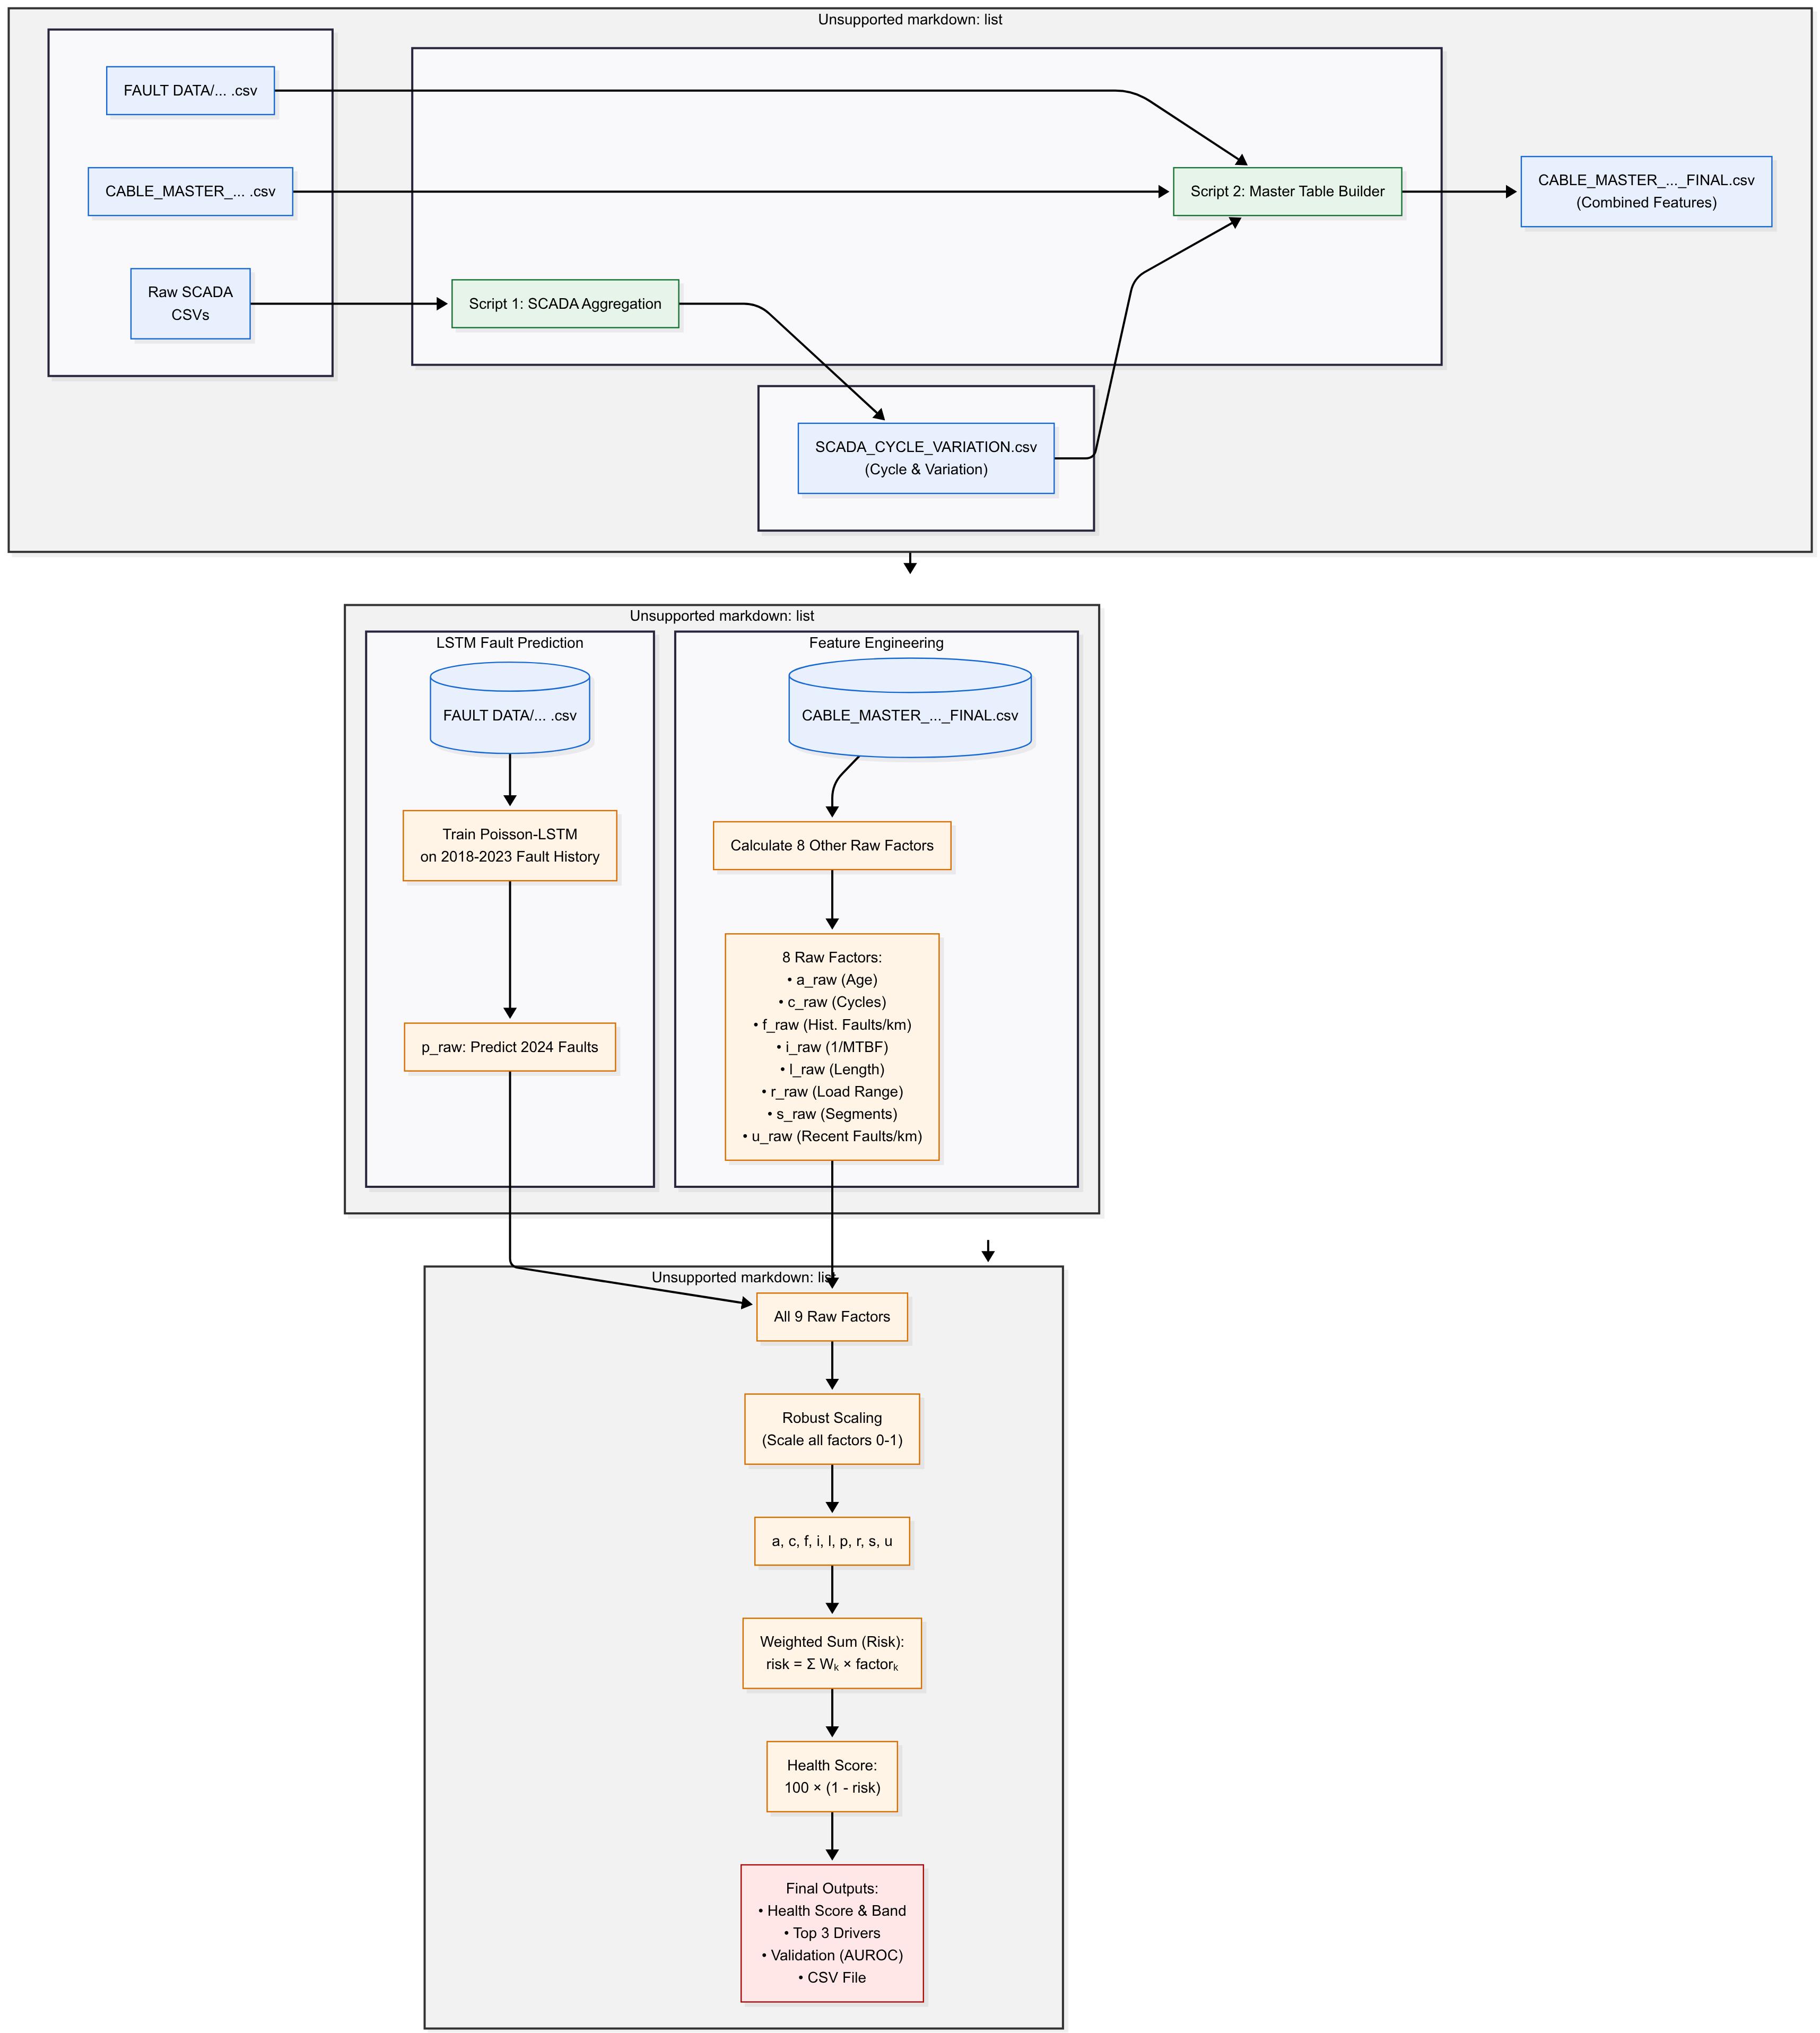
\includegraphics[width=1.1\linewidth, height = 1.5\linewidth, keepaspectratio]{fffff.png}
    \caption{The project workflow: from raw data ingestion and processing, through ML-based fault prediction, to the final calculation of the 9-factor Health Score.}
\end{figure}

\subsection{Step 1: SCADA Data Aggregation}
\begin{columns}[T]
    \begin{column}{0.5\textwidth}
        \begin{block}{Input}
            Raw, time-series SCADA data from multiple CSV files.
        \end{block}
        \begin{block}{Process}
            A Python script uses parallel processing to:
            \begin{itemize}
                \item Calculate daily peak-to-peak current variation.
                \item Count high-load "cycles" per month.
            \end{itemize}
        \end{block}
        \begin{block}{Output}
            \texttt{SCADA\_CYCLE\_VARIATION.csv}
        \end{block}
    \end{column}
    \begin{column}{0.5\textwidth}
        \begin{block}{Key SCADA Aggregations}
            The script processes the raw current readings to extract two key metrics for each cable per month:
            \begin{itemize}
                \item \textbf{Average Daily Variation:} It finds the difference between the maximum and minimum current for each day, and then averages these daily variations over the month. This measures the typical daily stress on the cable.
                \item \textbf{High-Load Cycles:} It counts how many times the current exceeded a high-load threshold during the month. This quantifies how often the cable was under significant strain.
            \end{itemize}
        \end{block}
    \end{column}
\end{columns}

\subsection{Step 2: Building the Master Table}
\begin{alertblock}{Goal: Create One Master File}
    The second script joins multiple data sources to create the final feature set.
\end{alertblock}
\vspace{1em}
\textbf{Inputs Joined:}
\begin{itemize}
    \item Cable asset data
    \item Aggregated SCADA data
    \item Historical fault records
\end{itemize}
\vspace{1em}
\textbf{Key Transformations:}
\begin{itemize}
    \item Aggregating fault counts \& MTBF.
    \item Extracting cable path from comments.
    \item Merging all tables on Switch ID.
\end{itemize}

\begin{block}{Output}
    \texttt{CABLE\_MASTER\_COMBINED\_FULL\_FINAL.csv}
\end{block}
\newpage

% --- Section 3: ML Model & Health Score ----------------------------------
\section{ML Model \& Health Score}

\subsection{Fault Prediction Process}
This diagram illustrates the process of using historical data to train the ML model, which then forecasts the probability of failure for each individual cable for the year 2024.
\begin{figure}[h!]
    \centering
    % FIXED: Corrected filename to remove space. Ensure your file is named "flowpredicted.png".
    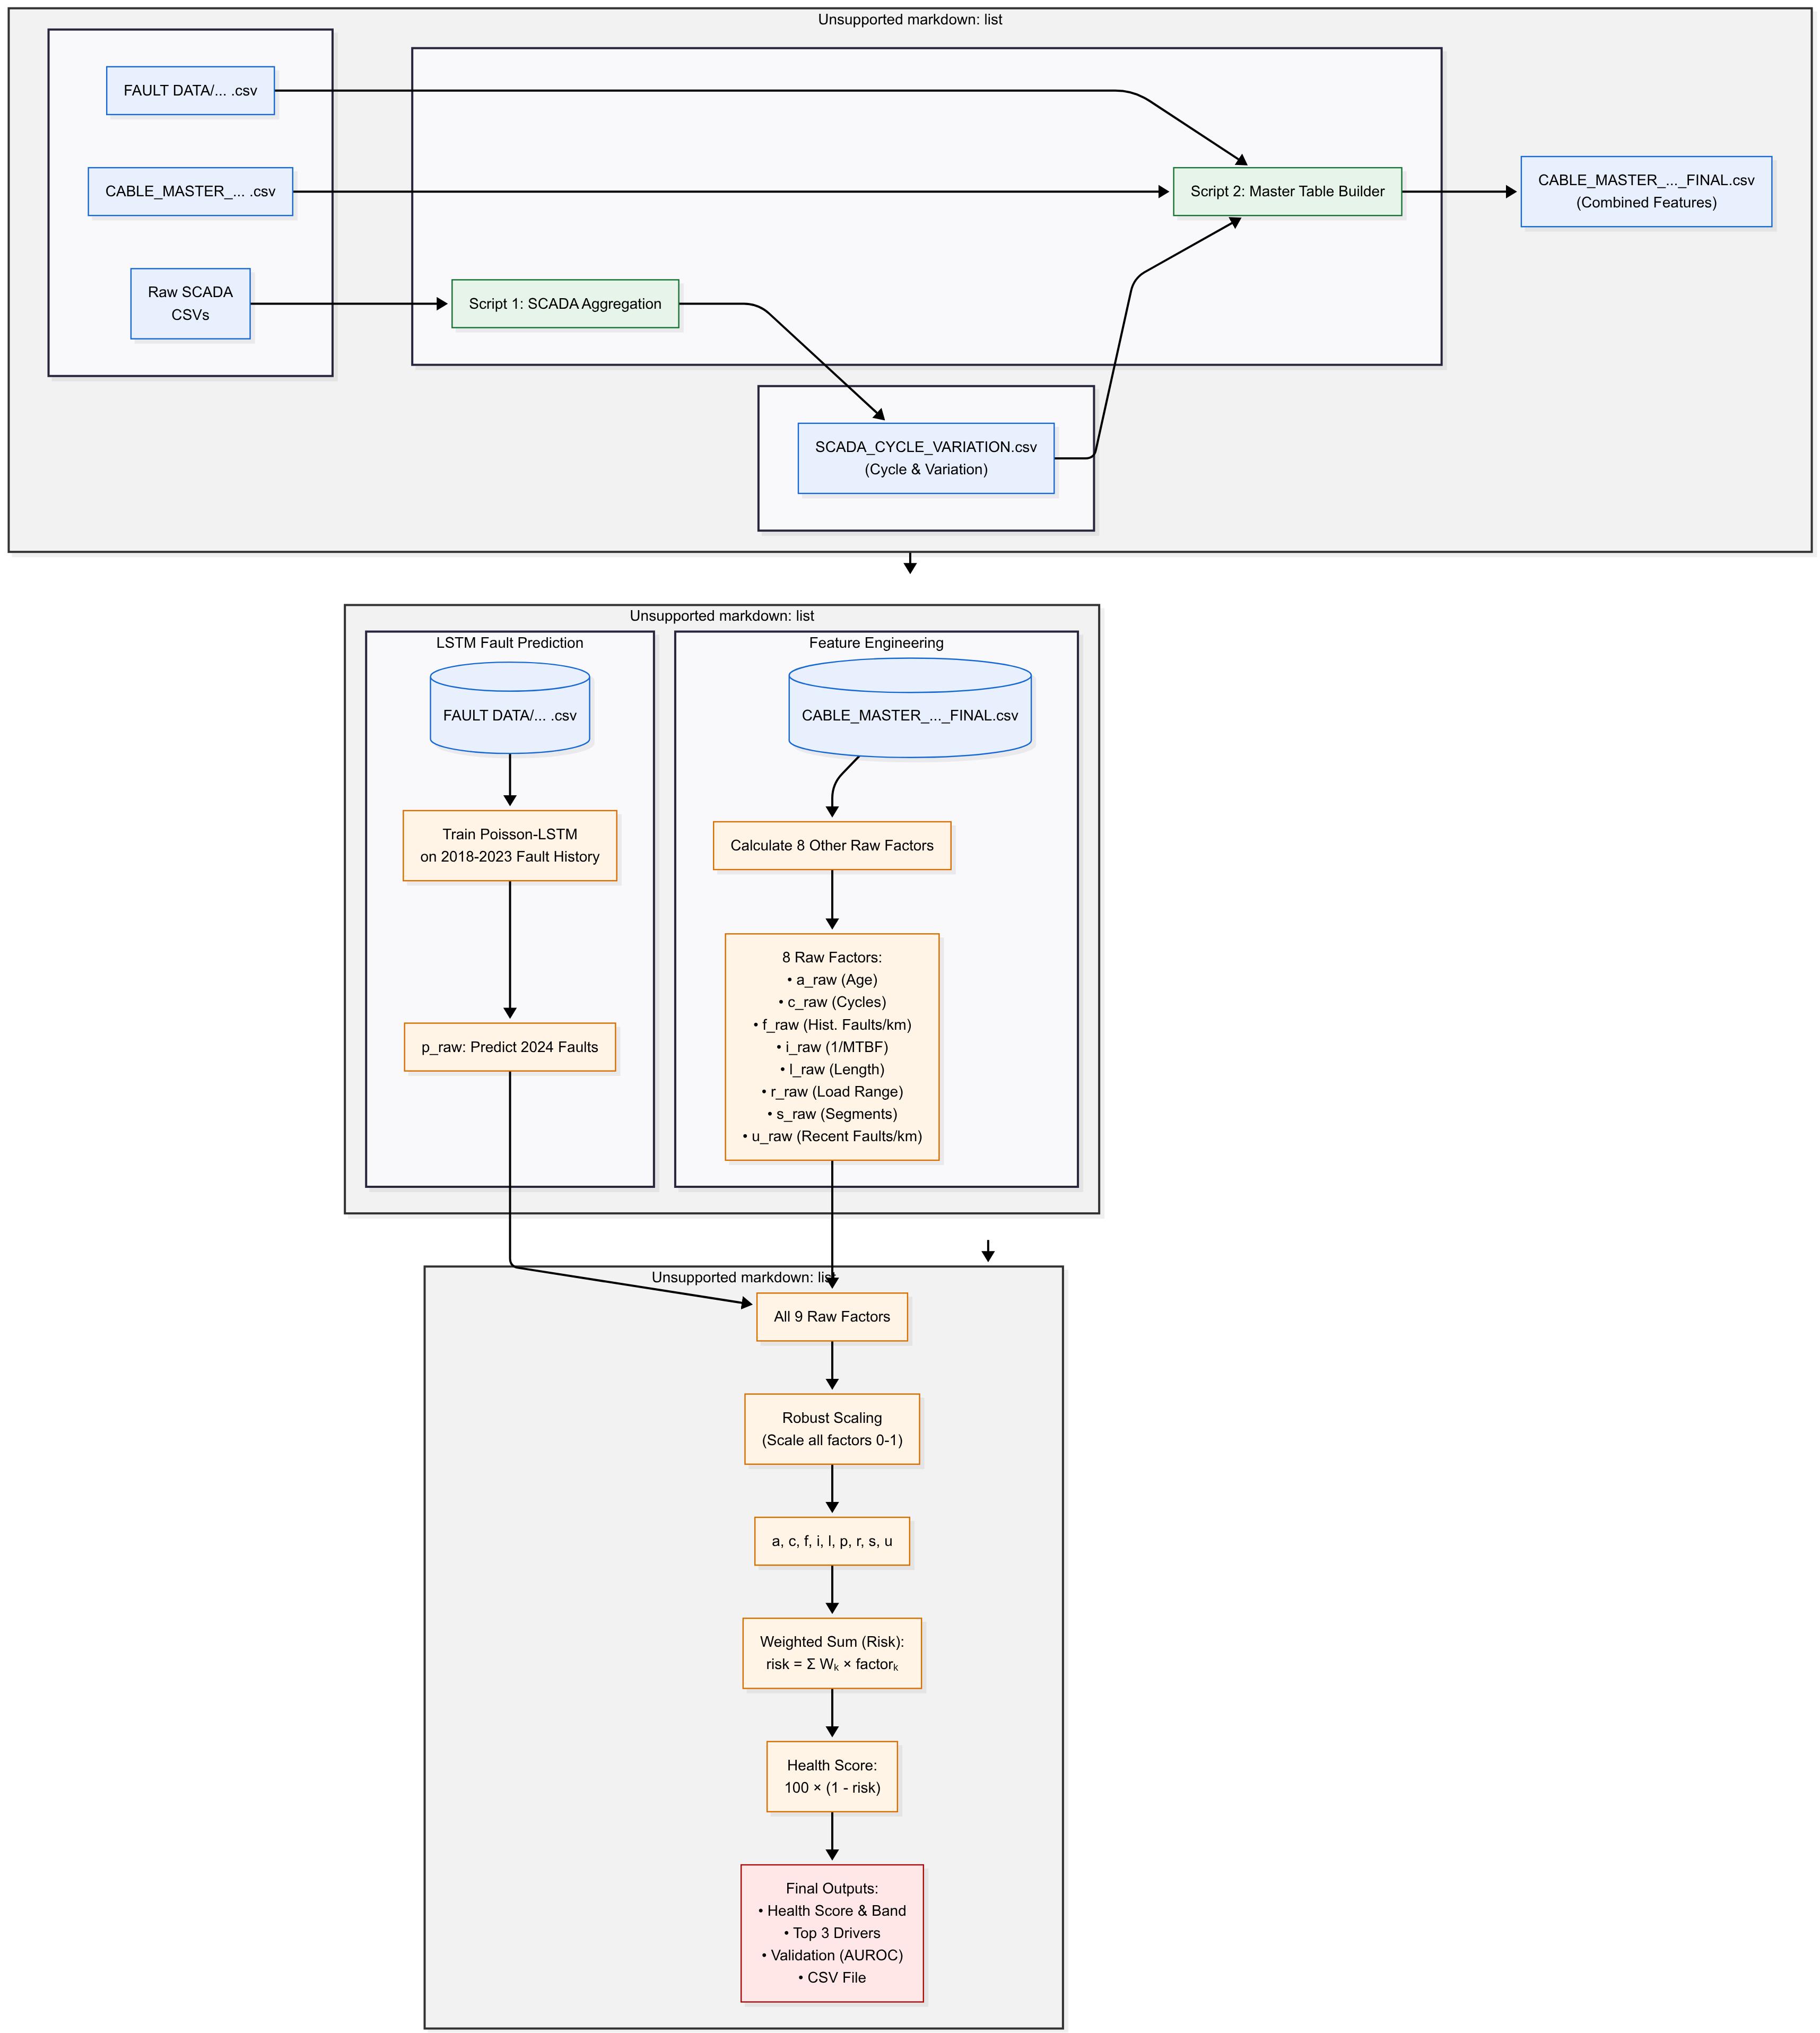
\includegraphics[width=1.1\linewidth, keepaspectratio]{fffff.png}
    \caption{Process flow for predicting 2024 cable faults using the trained ML model.}
\end{figure}


\subsection{The 9 Factors of Cable Health}
The health score is a weighted combination of 9 distinct risk factors.
\begin{columns}
    \begin{column}{0.5\textwidth}
        \textbf{Asset \& Operational Factors:}
        \begin{itemize}
            \item \textbf{a}: Age
            \item \textbf{l}: Length (log)
            \item \textbf{s}: Segments / Joints
            \item \textbf{c}: Cyclic Loading (SCADA)
            \item \textbf{r}: Load Range (SCADA)
        \end{itemize}
    \end{column}
    \begin{column}{0.5\textwidth}
        \textbf{Fault History \& Prediction:}
        \begin{itemize}
            \item \textbf{f}: Historical Faults / km
            \item \textbf{i}: Interruption Frequency (1/MTBF)
            \item \textbf{u}: Recent Faults (last 8-mo)
            \item \textbf{\textcolor{red}{p}}: \textbf{Predicted Faults (ML Model)}
        \end{itemize}
    \end{column}
\end{columns}
\begin{alertblock}{Key Innovation}
    The model doesn't just rely on the past; it uses an LSTM network to \textbf{forecast future faults}, which becomes a key factor (`p`).
\end{alertblock}

\subsection{Health Score Calculation Logic}
This diagram shows how the 9 scaled factors are combined using specific weights to produce a single risk value, which is then converted into the final Health Score from 0 to 100.
\begin{figure}[h!]
    \centering
    % FIXED: Corrected filename to remove space. Ensure your file is named "flowworking.png".
    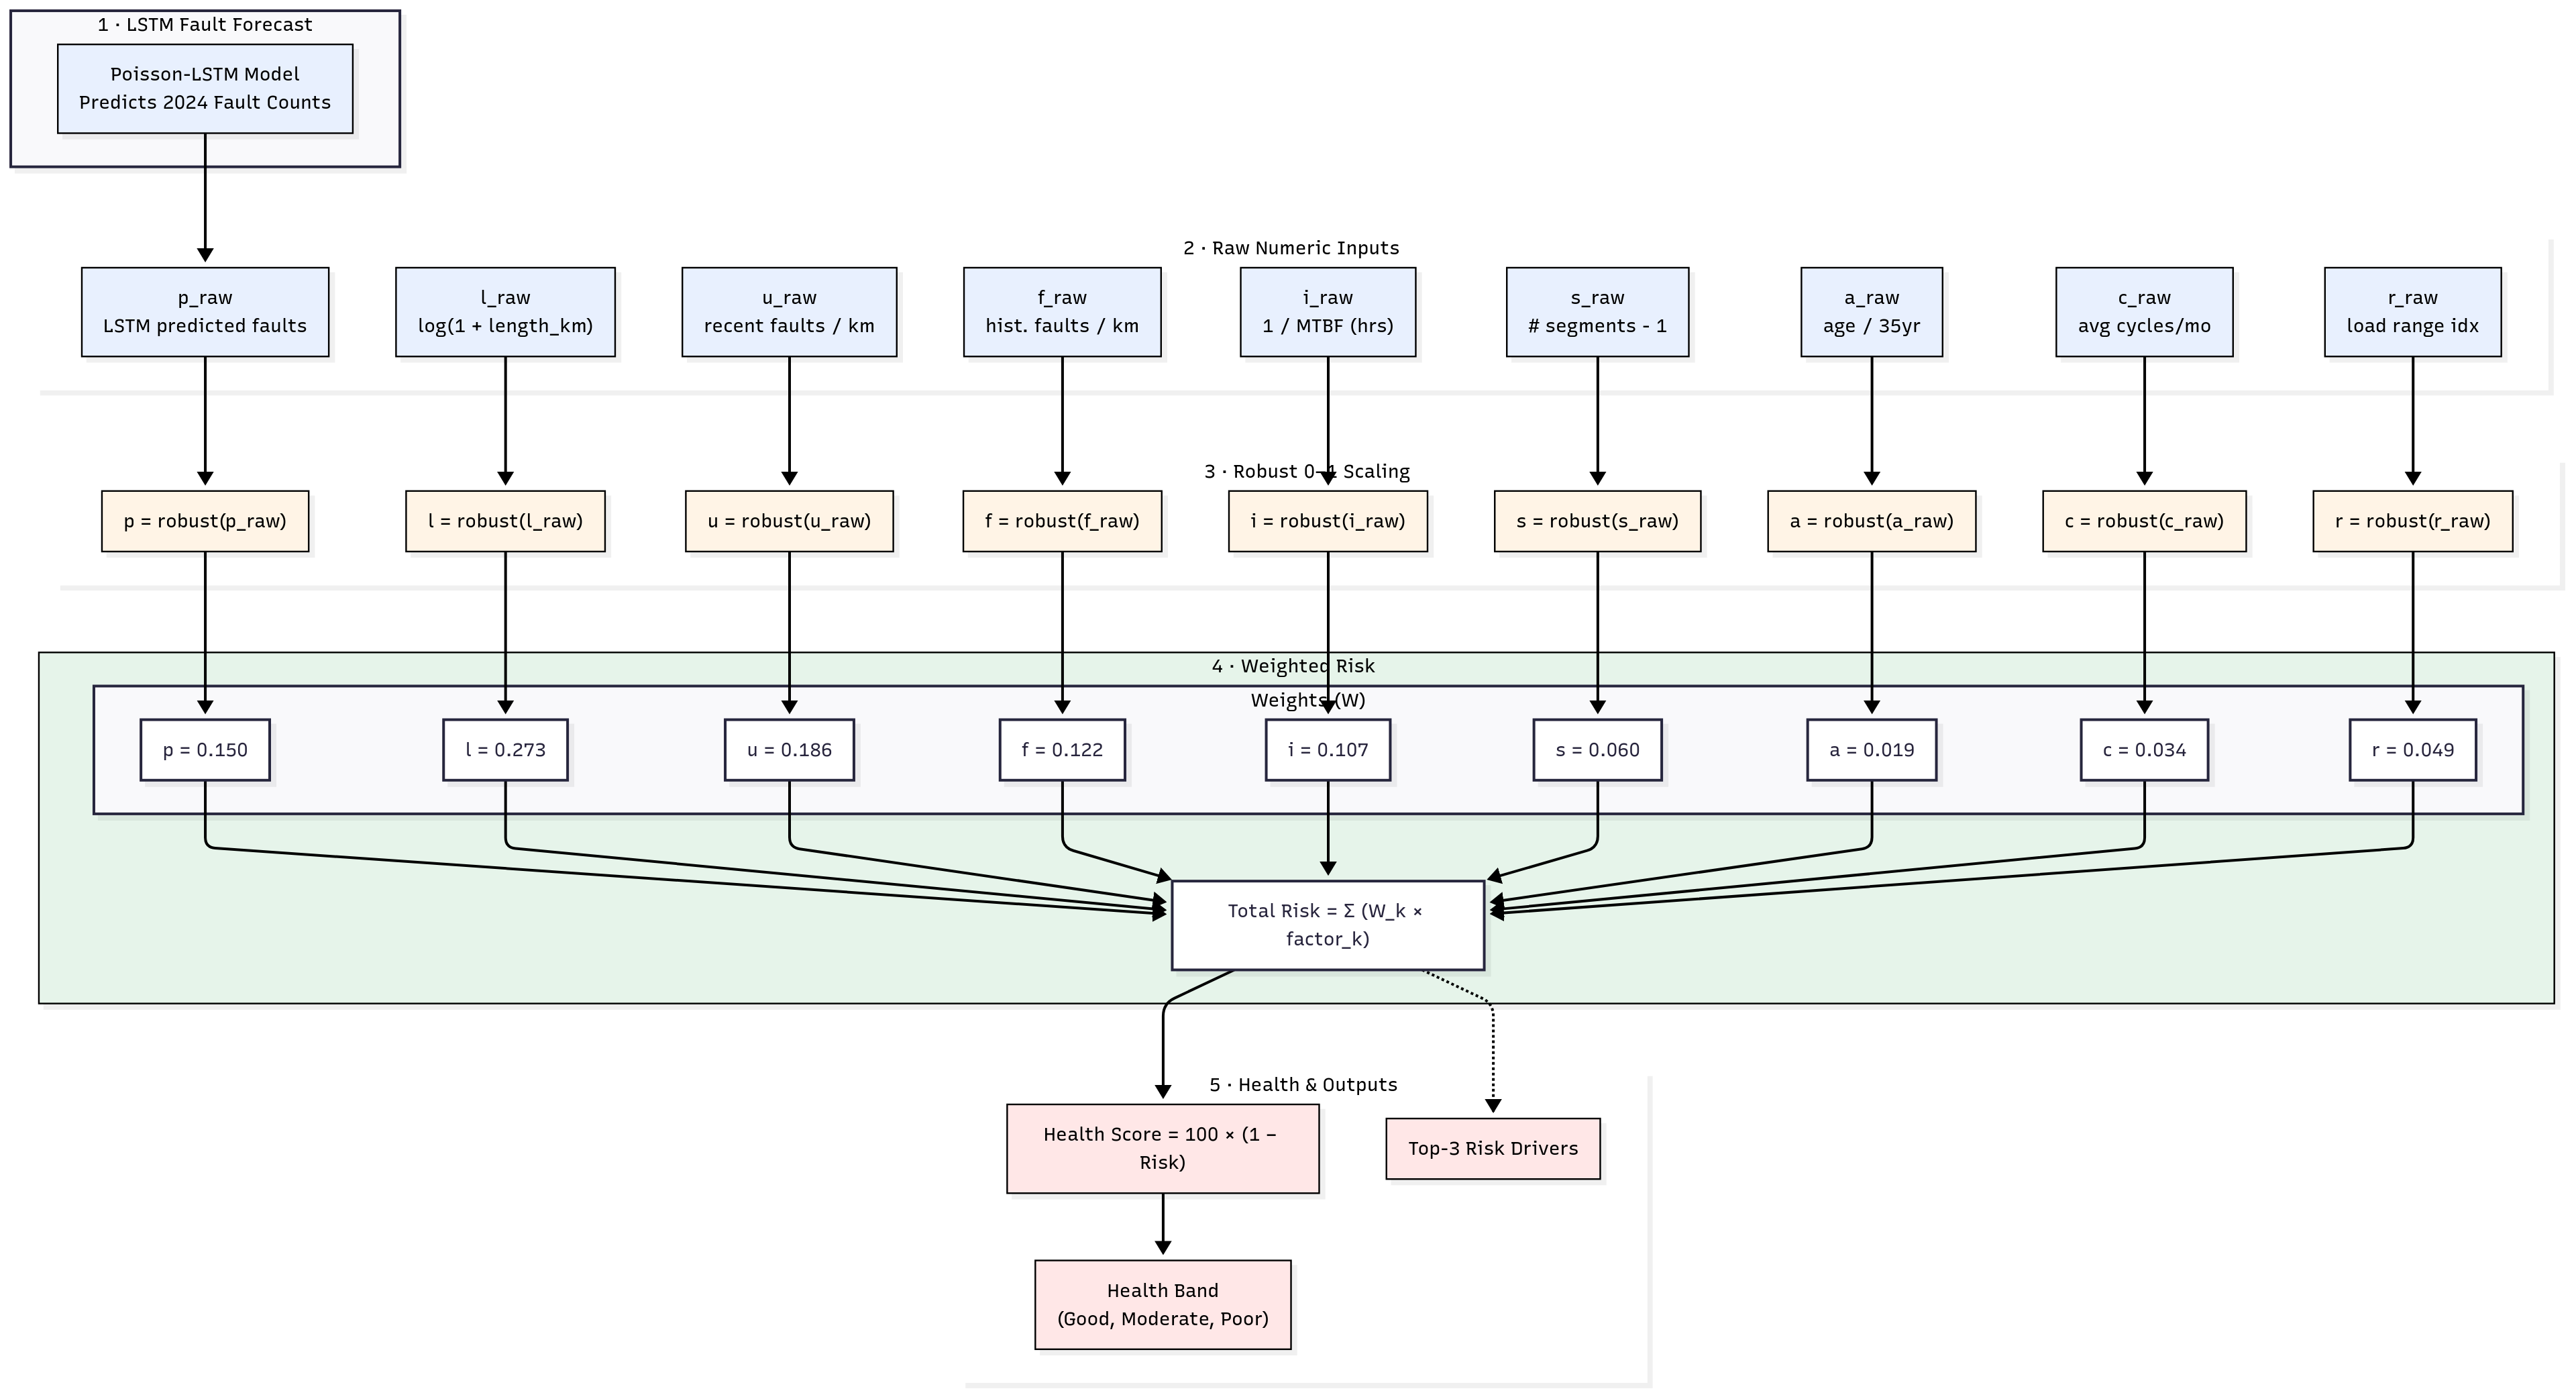
\includegraphics[width=\textwidth, height = \textwidth, keepaspectratio]{flow working.png}
    \caption{The logic for combining the 9 factors into a final Health Score.}
\end{figure}

\subsection{Understanding the Risk Factors}
\begin{itemize}
    \item \textbf{Age (a):} Date installed/35.
    \item \textbf{Length (l):} log(1+length-km). 
    \item \textbf{Segments (s):} from HT cable analyze the segment based on the JT NO 1B - JT NO 2B it is the one segment.
    \item \textbf{Cyclic Loading (c):} Frequent, large changes in load cause thermal stress. \\
    \textit{\small Example: cycle count is if one cable have 10 median load than how many number of times is going greater than 10 *1.6 or lower than 10/1.6 and aggregate all days within all months.  A cable with 20 high-load events (cycle count = 20) in a month is riskier than a cable with a steady load (cycle count = 0).}
    \item \textbf{Load Range (r):} The average daily variation between min/max current indicates thermal stress. \\
    \textit{\small Example: daily variation = daily daily max - daily min. aggregate and take mean for all each month}
    
    \item \textbf{Faults/km (f):} Normalizes fault history by cable length. \\
    \textit{\small Example: A 2km cable with 4 faults (2 faults/km) is riskier than a 5km cable with 5 faults (1 fault/km).}
    \item \textbf{Interruption Freq (i):} Inverse of Mean Time Between Failures (MTBF). \\
    \textit{\small Example: A cable failing every 2 years (0.5 freq) is riskier than one failing every 10 years (0.1 freq).}
    \item \textbf{Recent Faults (u):} Gives more weight to failures that happened recently. \\
    \textit{\small Example: A fault 3 months ago contributes more risk than one 3 years ago.}
    \item \textbf{Predicted Faults (p):} The ML model's forecast for faults in the next 12 months.
\end{itemize}
\newpage

\subsection{Final Score Calculation Steps}
\begin{block}{Step 1: Robust Scaling}

    \begin{itemize}
        \item \textbf{Sets Boundaries:} It defines the "minimum" as the 5th percentile and the "maximum" as the 95th percentile of the data
        \item \textbf{Clips Outliers:}  Any data point below the 5th percentile is treated as the minimum (scaled to 0). Any point above the 95th percentile is treated as the maximum (scaled to 1).
        \item \textbf{ Scales Everything Else:}  All the data between these percentiles is scaled proportionally to fit within the 0-1 range.
    \end{itemize}
\end{block}


\begin{block}{Step 2: Weighted Risk Calculation}
A weighted sum of the scaled factors produces a final risk value.
    $risk = \sum_{k \in \{a,c,f,...\}} W_k \times \text{factor}_k$
\end{block}

\begin{alertblock}{Step 3: Health Score}
    The final score is a simple transformation of the risk, from 0 (highest risk) to 100 (perfect health).
    $\text{Health Score} = \text{round}(100 \times (1 - \text{risk}))$
\end{alertblock}

\begin{block}{Output}
    \texttt{CABLE\_HEALTH\_SCORE\_2024.csv}
\end{block}
% --- Section 4: Results --------------------------------------------------
\section{Results \& Validation}

\subsection{Model Performance (2024 Validation)}
\begin{block}{From Health Score to a Prediction}
    To validate the score, we must define a cutoff. We categorize the score into bands and flag cables that are not "Good":
    \begin{itemize}
        \item \textbf{Poor (0-32)} or \textbf{Moderate (33-62)} $\rightarrow$ Predicted to Fail (Positive Class)
        \item \textbf{Good (63-100)} $\rightarrow$ Predicted to be Healthy (Negative Class)
    \end{itemize}
\end{block}
\begin{columns}[T]
    \begin{column}{0.5\textwidth}
        \begin{block}{Confusion Matrix}
        This matrix compares our predictions against the actual faults in 2024. From the values in the matrix, we calculate the model's sensitivity.
        \begin{figure}[h!]
            \centering
            % --- PLACEHOLDER FOR CONFUSION MATRIX IMAGE ---
            % Example: \includegraphics[width=0.8\linewidth]{confusion_matrix.png}
            \fbox{
                    \centering
                    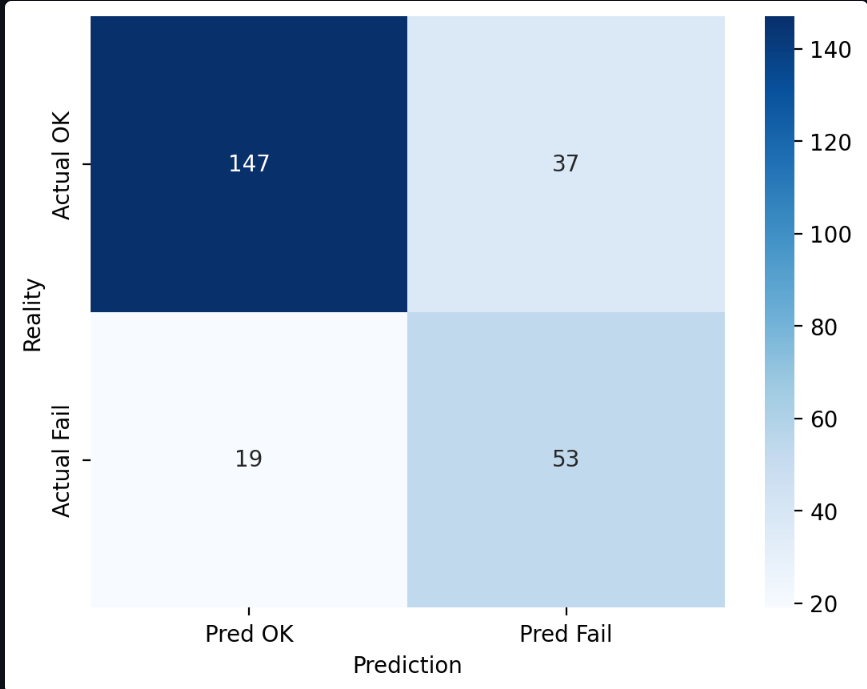
\includegraphics[width=0.6\linewidth , height = 0.4\linewidth]{confusion.png}
            }
            \caption{Confusion Matrix for 2024 Validation.}
        \end{figure}
        \textbf{Sensitivity (Recall):} $\approx \textbf{78\%}$
        \end{block}
    \end{column}
\end{columns}
    \begin{columns}[T]
    \begin{column}{0.5\textwidth}
     \begin{block}{Key Performance Metrics}
         The confusion matrix compares our predictions (cables flagged as 'Poor' or 'Moderate') against the actual outcomes in 2024.

         \begin{itemize}
             \item \textbf{Accuracy: 75.4\%} \\
             \textit{\small Overall, how often is the model correct?} \\
             Formula: $\frac{TP+TN}{Total} = \frac{54+139}{256}$
             
             \item \textbf{Precision: 54.5\%} \\
             \textit{\small When it predicts a failure, how often is it right?} \\
             Formula: $\frac{TP}{TP+FP} = \frac{54}{54+45}$
             
             \item \textbf{Sensitivity (Recall): 75.0\%} \\
             \textit{\small Of all actual failures, what fraction did we identify?} \\
             Formula: $\frac{TP}{TP+FN} = \frac{54}{54+18}$
         \end{itemize}
     \end{block}
   \end{column}
    \begin{column}{0.5\textwidth}
        \begin{alertblock}{Intuition}
        A sensitivity of 78\% means: \textbf{By focusing on cables with "Poor" or "Moderate" health, we would have successfully preempted 78\% of all the failures that occurred in 2024.}
        \end{alertblock}
        \vspace{1em}

    \end{column}
\end{columns}



\end{document}